% =============================================================================
% sections/design/drone/physical_design/drone_overview.tex  -  Drone Overview
% Teams: drone (best guess - unconfirmed) / Status: EXAMPLE (scope approximation)
%
% EXAMPLE CONTENT for scope/layout approximation - not final report text.
% Scope covers the Drone's physical dimensions, overall configuration, and
% operational parameters relevant to autonomous target searching. Marked with
% \exampleflag on its heading in the assembler.
% =============================================================================

\todo[inline]{Jury feedback (Preliminary, O/PRR-030c): the drone was never
actually shown despite an extensive description. Add real photos of the
assembled drone here, before or alongside the architecture diagram
(evidence-first rule).}

The Drone is a quadcopter built from Commercial Off-The-Shelf (COTS)
components. \autoref{fig:drone_electronics_architecture} provides a
high-level view of its onboard electronics architecture and subsystem
interfaces: the Core Avionics Subsystem, Navigation Subsystem, Perception
\& Video Subsystem, Communication Segment, and Propulsion Subsystem.

\begin{figure}[!htbp]
    \centering
    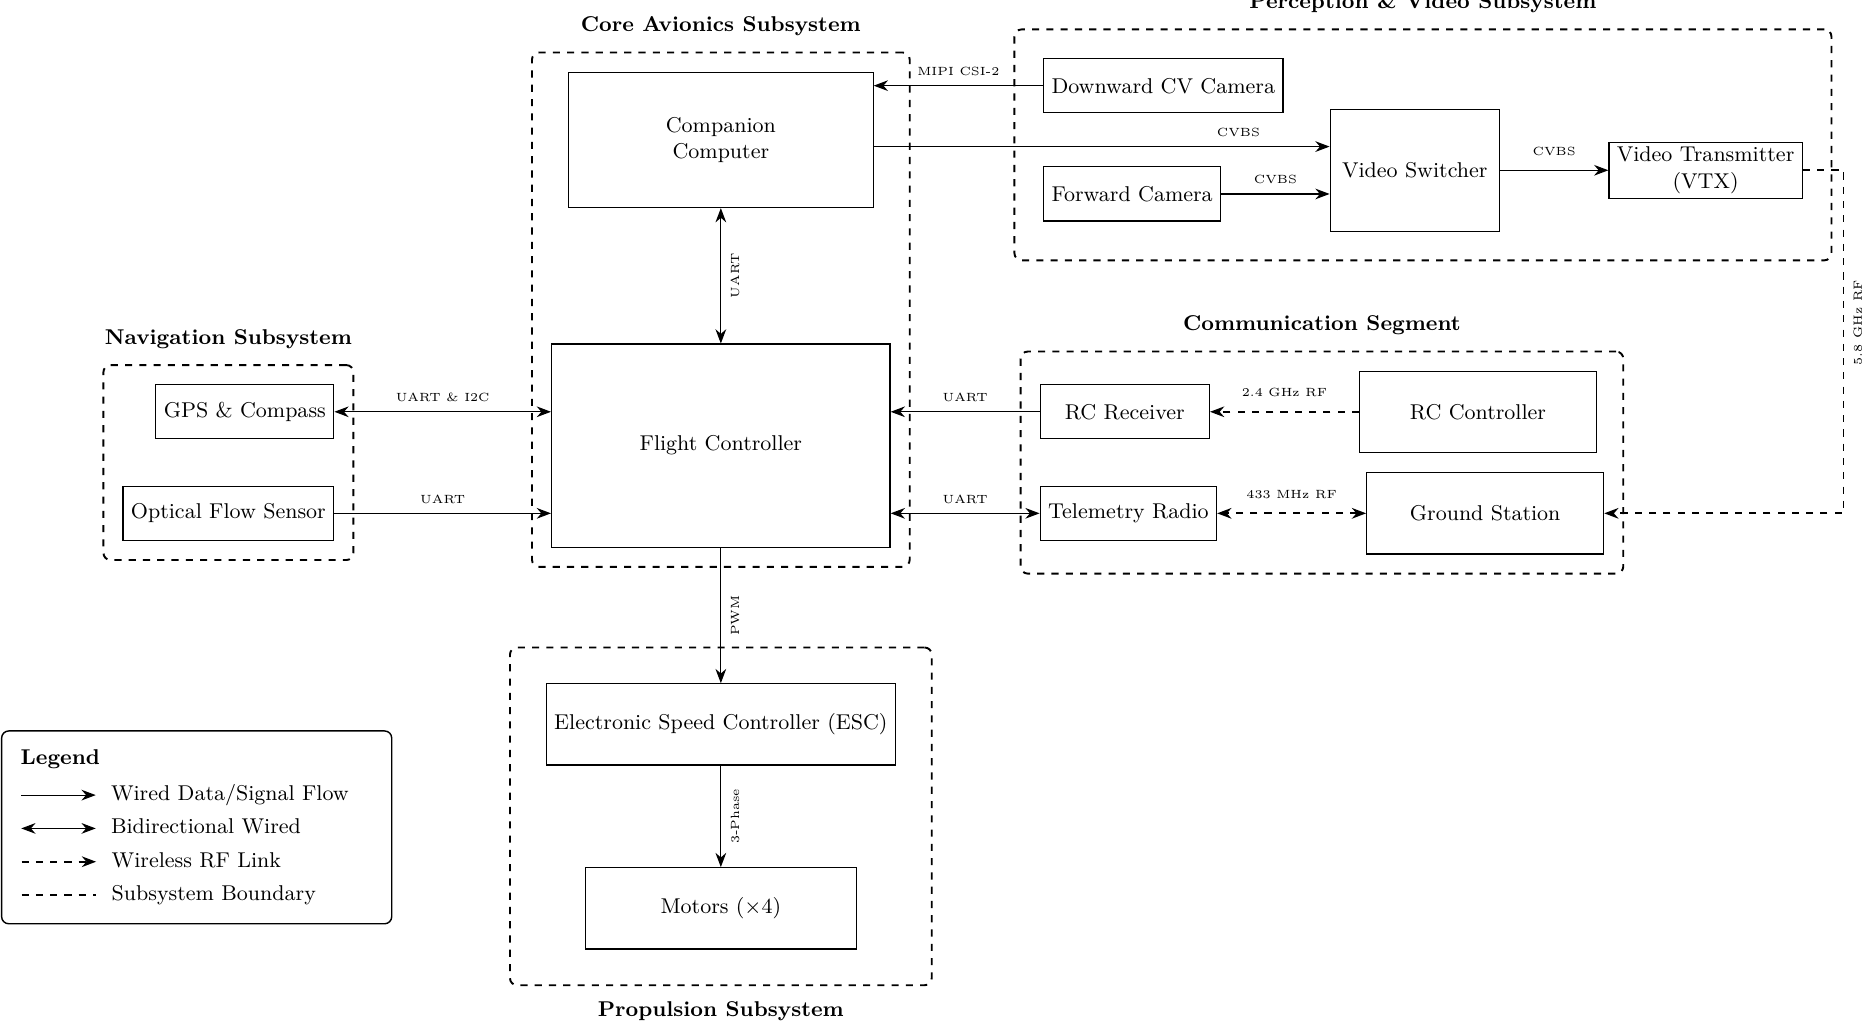
\includegraphics[width=0.85\linewidth]{teams/drone/figures/drone_electronics_architecture}
    \caption{High-level Drone electronics architecture and subsystem interfaces}
    \label{fig:drone_electronics_architecture}
\end{figure}
